% !TEX root = /home/fred-olav/afgv/book/
\chapter{Analog electronic instrumentation}

An ``analog'' electronic signal is a voltage or current proportionate to the value of some physical measurement or control quantity.  An instrument is often classified as being ``analog'' simply by virtue of using an analog signal standard to communicate information, even if the internal construction and design of the instrument may be mostly digital in nature.  This is to distinguish such instruments from those making use of no analog electronic signals at all (e.g. wireless or Fieldbus instruments).

\section{4 to 20 mA analog current signals}

The most popular form of signal transmission used in modern industrial instrumentation systems (as of this writing) is the 4 to 20 milliamp DC standard.  This is an \textit{analog} signal standard, meaning that the electric current is used to proportionately represent measurements or command signals.  Typically, a 4 milliamp current value represents 0\% of scale, a 20 milliamp current value represents 100\% of scale, and any current value in between 4 and 20 milliamps represents a commensurate percentage in between 0\% and 100\%.  The following table shows the corresponding current and percentage values for each 25\% increment between 0\% and 100\%.  Every instrument technician tasked with maintaining 4-20 mA instruments commits these values to memory, because they are referenced so often: \index{4 to 20 mA}

% No blank lines allowed between lines of an \halign structure!
% I use comments (%) instead, so that TeX doesn't choke.

$$\vbox{\offinterlineskip
\halign{\strut
\vrule \quad\hfil # \ \hfil & 
\vrule \quad\hfil # \ \hfil \vrule \cr
\noalign{\hrule}
%
% First row
\textbf{Current value} & \textbf{\% of scale} \cr
%
\noalign{\hrule}
%
% Another row
4 mA & 0\% \cr
%
\noalign{\hrule}
%
% Another row
8 mA & 25\% \cr
%
\noalign{\hrule}
%
% Another row
12 mA & 50\% \cr
%
\noalign{\hrule}
%
% Another row
16 mA & 75\% \cr
%
\noalign{\hrule}
%
% Another row
20 mA & 100\% \cr
%
\noalign{\hrule}
} % End of \halign 
}$$ % End of \vbox

\filbreak

For example, if we were to calibrate a 4-20 mA temperature transmitter for a measurement range of 50 to 250 degrees C, we could relate the current and measured temperature values on a graph like this:

$$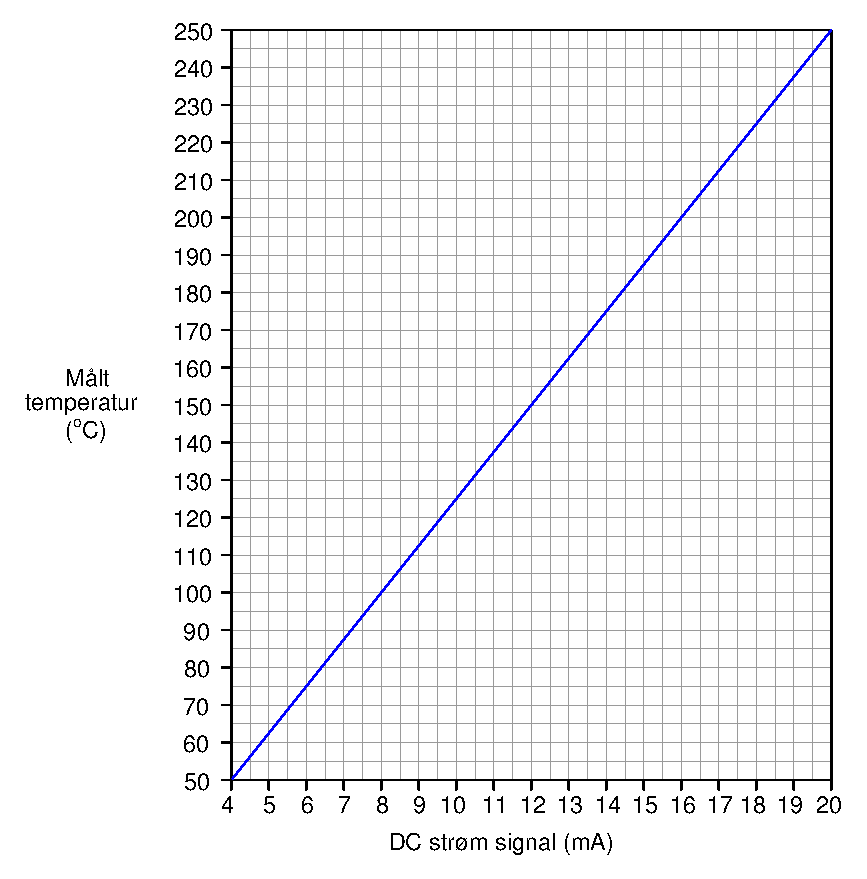
\includegraphics{current01.eps}$$

This is not unlike 3-15 pounds per square inch (PSI) pneumatic signal standard, where a varying air pressure signal proportionately represents some process variable.  Both 3-15 PSI and 4-20 mA signal standards are referred to as \textit{live zero} because their ranges begin with a non-zero value.  This ``live'' zero provides a simple means of discriminating between a legitimate 0\% signal value and a failed signal (e.g. leaking tube or severed cable)\footnote{Not all industrial measurement and control signals are ``live zero'' like the 3-15 PSI and 4-20 mA standards.  0 to 10 volts DC is a common ``dead zero'' signal standard, although far more common in environmental (building heating and cooling) control systems than industrial control systems.  I once encountered an old analog control system using $-10$ volts to +10 volts as its analog signal range, which meant 0 volts represented a 50\% signal!  A failed signal path in such a system could have been very misleading indeed, as a 50\% signal value is not suspicious in the least.}.  \index{Live zero}

\filbreak

An important concept to grasp with all analog instrumentation is that instruments sending and receiving analog signals must be compatibly ranged in order to properly represent the desired variable.  To illustrate, let us consider a temperature measurement system consisting of a thermocouple\footnote{This is a temperature sensing element consisting of two different metal wires joined together, which generate a small voltage proportional to temperature.  The correspondence between junction temperature and DC millivoltage is very well established by scientific testing, and so we may use this principle to sense process temperature.}, a temperature transmitter, a 250 ohm resistor (to convert the 4-20 mA analog signal into a 1-5 volt analog signal), and a special voltmeter functioning as a temperature indicator:

$$\includegraphics{current60.eps}$$

Note how the output range of each sending device matches the input range of its corresponding receiving device.  If we view this system as a path for information to flow from the thermocouple's tip to the transmitter to the resistor and finally to the voltmeter/indicator, we see that the analog output range of each device must correspond to the analog input range of the \textit{next} device, or else the real-world meaning of the analog signal will be lost.  

This correspondence does not happen automatically, but must be established by the instrument technician building the system.  In this case, it would be the technician's responsibility to properly adjust the range of the temperature transmitter, and also to ensure the indicator's display scale was properly labeled.  Both the thermocouple and the resistor are non-adjustable devices, their input/output characteristics being fixed by physical laws.
  
\vskip 10pt

\filbreak

DC current signals are also used in control systems to command the positioning of a final control element, such as a control valve or a variable-speed motor drive (VSD).  In these cases, the milliamp value does not directly represent a process measurement, but rather how the degree to which the final control element influences the process.  Typically (but not always!), 4 milliamps commands a closed (shut) control valve or a stopped motor, while 20 milliamps commands a wide-open valve or a motor running at full speed.  Final control elements often are equipped with adjustable ranges so that an accurate correspondence between the analog signal and the desired control action may be ensured.

\vskip 10pt

Thus, most industrial control systems use at least \textit{two} different 4-20 mA signals: one to represent the process variable (PV) and one to represent the command signal to the final control element (the ``manipulated variable'' or MV):

$$\includegraphics{current02.eps}$$

The relationship between these two signals depends entirely on the response of the controller.  There is no reason to ever expect the PV and MV current signals to be equal to each other except by chance, for they represent entirely different variables.  In fact, if the controller is reverse-acting, it is entirely normal for the two current signals to be inversely related: as the PV signal increases going to a reverse-acting controller, the output signal will decrease.  If the controller is placed into ``manual'' mode by a human operator, the output signal will have no automatic relation to the PV signal at all, instead being entirely determined by the operator's whim.






\filbreak
\section{Sammenhengen mellom 4-20mA signal og andre signaler}


Et 4-20mA strømsignal representerer et eller annet signal fra 0 100\%. Denne sammenhengen er vanligvis lineær. 

$$\includegraphics{current42.eps}$$

\label{instrument_range_linear_equation}

Siden dette er en lineær funksjon, kan vi bruke formelen for en rett linje til å relatere rett signal \% til strømverdier.


$$y = mx + b$$

\noindent
Hvor,

$y$ = Utgangen fra instrumentet

$x$ = Inngangen fra instrumentet

$m$ = Stigningstallet for linjen

$b$ = $y$-skjeringspunktet (m.a.o. \textit{aktivt} nullpunkt for instrumentutgangen. \index{aktivt nullpunkt}) Denne vil vi kalle $y_{start}$ fra nå av. 
\vskip 10pt

Med en gang vi har passende verdier for $m$ og $y_{start}$, kan vi bruke formelen for en rett linje for å konvertere mellom inn og utgangen på en transmitter. 

Før vi kan bruke formelen må vi finne verdiene for stigningstallet og y-skjæringspunktet for den transmitteren vi jobber med.  

For den lineære funksjonen som vises skal vi finne stigningstallet ($m$) ved å dele linjens $y_{range}$ med linjens $x_{range}$. $y_{range}$ er transmitterens inngangsområde, og $x_{range}$ er transmitteres utgangsområde. 

$$\includegraphics{current43.eps}$$

$$m =\dfrac{ y_{range}} {x_{range}} = \dfrac {20 - 4} {100 - 0} = \dfrac{ 16} {100}$$

Dette gir:

$$y = \left({16 \over 100}\right)x + y_{start}$$

For å finne skjæringspunktet med y-aksen ($b$), må vi løse denne ligningen for noen kjente verdier av $(x,y)$. Vi kjenner verdiene i starten og enden av måleområde, og kan velge det vi vil. Vi velger starten med $(x,y) = (0,4)$. 

\begin{align*}
	4 &= \left({16 \over 100}\right)0 + y_{start}\\
	4 &= 0 + b\\
	b &= 4
\end{align*}
\vskip 10pt


Nå har vi en komplett formel for å konvertere en prosentverdi om til en milliampere verdi:


$$y = \left({16 \over 100}\right)x + 4$$

Vi kan nå bruke denne formelen for å regne ut hvor mange milliamper en gitt prosent inngangssignal tilsvarer. Vi kan f.eks. bruke et inngangsignal på 34.7\% til å regne ut tilhørende milliamper verdi:

\begin{align*}
	y &= \left({16 \over 100}\right)34.7 + 4\\
	y &= 5.552 + 4\\
	y &= 9.552
\end{align*}
Vi ser altså at 34.7\% er det samme som 9.552 mA i 4-20 mA signalområdet. 

\vskip 10pt

Denne formelen kan brukes til alle lineære instrumenter. Men om vi har forsøvet nullpunkt på instrumentaksen $x$ kreves ofte flere mellom regninger.

\vskip 10pt 
Mange elever foretrekker å bruke en grafisk representasjon av de to måleområdene vi skal konvertere mellom. 

$$\includegraphics{current63.eps}$$

Ut fra denne representasjonen kan vi sette opp følgende formel for konvertering mellom signaler. 
	\begin{align*}
		\dfrac{y-y_{start}}{y_{range}}&=\dfrac{x-x_{start}}{x_{range}}\\
	\end{align*}

Merk her at $y_{range}$ og $x_{range}$ regnes ut fra måleområde slutt til måleområde start. 

For en transmitter som 4mA som nullpunkt blir det (20-4=16), mens for en transmitter med 20mA som nullpunkt blir det (4-20=-16). 

Vi kan også sette opp denne formelen med rene transmitter begreper:

$$\includegraphics{current59.eps}$$




\filbreak
\subsection{Eksempel: Regulatorutgang til reguleringsventil.}

$$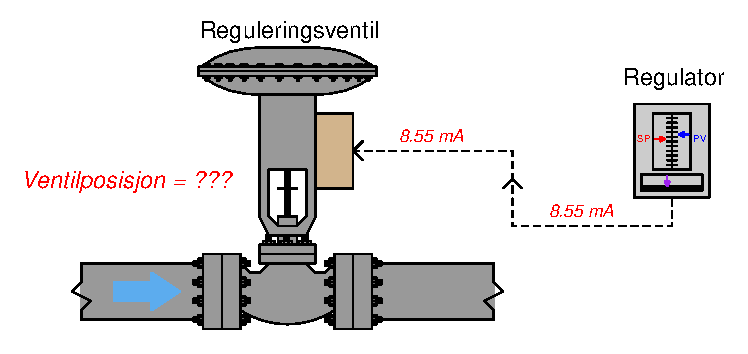
\includegraphics{current44.eps}$$

\noindent

\textit{En PID regulator sender et utgangsignal til en direkteverkende reguleringsventil (d.v.s 4mA er lukket og 20mA er helt åpen).Hvor åpen (0-100\%i) vil reguleringsventilen være med dette signalet?}


\vskip 10pt

For å løse utregningen med hensyn på  ventilutslag ($x$), bruker vi formelen som vi har kommet frem til tidligere. 

	\begin{align*}
		\dfrac{y-y_{start}}{y_{range}}&=\dfrac{x-x_{start}}{x_{range}}\\
		\\
		\dfrac{8.55-4}{16}&=\dfrac{x-0}{100}\\
		\\
		\dfrac{100 \cdot 4.55}{16}&=x\\
		\\
		x&={28.4}\\
	\end{align*}

Vi kan derfor forvente at reguleringsventilen er 28.4\% åpen når den får tilført 8.55mA


\filbreak
\subsection{Eksempel: Strømningsmåler}

$$\includegraphics{current45.eps}$$


\noindent
\textit{En strømningsmåler har et måleområde på 0 til 1400 liter per minutt. Regn ut strømsignalet med en strømningsrate på 816 l/m.}

\vskip 10pt

Vi velger strøm som $y$ i formelen og setter inn. 


	\begin{align*}
		\dfrac{y-y_{start}}{y_{range}}&=\dfrac{x-x_{start}}{x_{range}}\\
		\\
		\dfrac{y-4}{16}&=\dfrac{816-0}{1400}\\
		\\
		y&=\dfrac{816\cdot16}{1400}+4\\
		\\
		y&={13.3mA}\\
	\end{align*}

Vi ser at transmitteren skal sende ut en strøm på 13.3mA med en strømningsrate på 816 l/m. 

\vskip 10pt


\filbreak
\subsection{Eksempel: Temperaturtransmitter}

$$\includegraphics{current47.eps}$$

\noindent
\textit{En elektronisk temperaturtransmitter har et måleområde på 50-140°C, med en strømutgang på 4-20mA utgangssignal. Regn ut strømmen denne transmitteren sender ut når den måler en temperatur på 79°C.}

\vskip 10pt

Først kan vi sette opp en en oversikt med aksene parallelle. Dette kan vi gjøre for alle lineære konverteringer og det gir et mer kompakt over oversiktlig bilde av sammenhengen.  


$$\includegraphics[width=0.8\textwidth]{current48.eps}$$

Nå kan vi sette opp konverteringsformelen. 

	\begin{align*}
		\dfrac{y-y_{start}}{y_{range}}&=\dfrac{x-x_{start}}{x_{range}}\\
		\\
		\dfrac{y-4}{16}&=\dfrac{79-50}{90}\\
		\\
		y&=\dfrac{29\cdot16}{90}+4\\
		\\
		y&={9.2mA}\\
	\end{align*}




\filbreak
\subsection{Example calculation: pH transmitter}

$$\includegraphics[width=0.4\textwidth]{current49.eps}$$

\noindent
\textit{En pH transmitter er kalibrert for et måleområde på 4pH til 10pH, med et 4-20mA utgangssignal. Regn ut hvilken pH som måles når transmitteren sender en strøm på 11.3 mA. }

\vskip 10pt
Først setter vi opp en parallell oversikt over de to måleområdene. 

$$\includegraphics[width=0.4\textwidth]{current50.eps}$$

Så er det bare å sette inn i konverteringsformelen. 

	\begin{align*}
		\dfrac{y-y_{start}}{y_{range}}&=\dfrac{x-x_{start}}{x_{range}}\\
		\\
		\dfrac{y-4}{6}&=\dfrac{11.3-4}{16}\\
		\\
		y&=\dfrac{7.3\cdot6}{16}+4\\
		\\
		y&={6.74mA}\\
	\end{align*}

Transmitteren måler en pH på 6.7 når utgangen sender en strøm på 11.3 mA







\filbreak
\subsection{Eksempel: I/P omformer med reverserende utgangsignal}

$$\includegraphics{current51.eps}$$

%\noindent
\textit{En strøm til trykkomformer brukes for å konvertere 4-20mA strømsignal til et 3-15PSI pneumatisk signal. Akkurat denne transmitteren er konfigurert for å ha en reverserende utgang istedenfor direkte. Dette betyr at trykket på utgangen er 15PSI med en strøm på 4mA, og 3 PSI med 20mA. Regn ut hvilken strøm som sendes til omformeren når utgangen har et trykk på 12.7 PSI.}

\vskip 10pt

Reverserende instrumenter er fremdeles lineære, og vi kan verfor bruke samme oppsett som før. Legg merke til range på x-aksen som går fra 15 til 3 som gir en range på -12 ($3-15=-12$).

$$\includegraphics{current52.eps}$$

	\begin{align*}
		\dfrac{y-y_{start}}{y_{range}}&=\dfrac{x-x_{start}}{x_{range}}\\
		\\
		\dfrac{y-4}{16}&=\dfrac{12.7-15}{-12}\\
		\\
		y&=\dfrac{-2.3\cdot16}{-12}+4\\
		\\
		y&={7.1mA}\\
	\end{align*}



Strømmen som sendes til transmitteren er 7.1mA. 



\filbreak
\subsection{Eksempel: PLS analog inngang}


$$\includegraphics{current53.eps}$$

\noindent
\textit{En Allen-Bradley SLC500 PLS bruker en 16-bit analog-til-digital omformer i AI kortet 1746-NI4. I dette kortet konverteres 4-20 mA til digitale nummer(integere) fra 3277 (ved 4 mA) til 16384 (ved 20 mA). I en PLS-en skal denne verdien vises på det display (HMI). En verdi fra 3277-16384 vil ikke være særlig nyttig for en operatør. Derfor må disse verdiene skalleres ved å regne de om til 0-700 l/m. Utrenginger med integere er ikke serlig praktisk og vi må derfor først konvertere de til floating point datatyper. Finn en formel for utregningen og vis hvordan denne kan implementeres i PLS programmet.}

\vskip 10pt


We are already given the raw number values from the analog card's analog-to-digital converter (ADC) circuit for 4 mA and 20 mA: 3277 and 16384, respectively.  These values define the domain of our linear graph:

$$\includegraphics{current64.eps}$$

Vi kan nå sette opp konverteringsformelen:


	\begin{align*}
		\dfrac{y-y_{start}}{y_{range}}&=\dfrac{x-x_{start}}{x_{range}}\\
		\\
		\dfrac{y-0}{700}&=\dfrac{x-3277}{16384-3277}\\
		\\
		f(x)=y&=\dfrac{(x-3277)\cdot700}{13107}\\
	\end{align*}

Når vi skal lage PLS programmet følger vi regnerekkefølgen:

\begin{enumerate}
	\item Paranteser
	\item Potenser og røtter
	\item Multiplikasjon og divisjon
	\item Addisjon og subtraksjon

\end{enumerate}

Vi tar altså utgangpunkt  i den variable (x) og utfører følgende:

\begin{enumerate}
	\item Utregning i parantesen $x-3277$
	\item Multiplisering og dividering. Rekkefølgen er likegyldig eller den kan slåes sammen i en blokk. 
	\item Vi legger så resultatet inn i variabelen y som  kan brukes i HMI-en. 
\end{enumerate}


I pragrammet legger vi først inn en konverteringsblokk for så å legge blokker inn ut fra regnefekkefølgen.

%$$\includegraphics[width=0.8\textwidth]{current65.png}$$

En annen mulighet er å bruke en ferdig converteringsblokk, f.eks. LIN\_TRAFO fra util biblioteket til Codesys. 
%$$\includegraphics[width=0.8\textwidth]{current66.png}$$






\filbreak
\section{Controller output current loops}


The simplest form of 4-20 mA current loop is the type used to represent the output of a process controller, sending a command signal to a final control element.  Here, the controller supplies both the electrical power and signal information to the final control element, which acts as an electrical load.  To illustrate, consider the example of a controller sending a 4-20 mA signal to an I/P (current-to-pressure) signal converter, which then pneumatically drives a control valve:

$$\includegraphics{current03.eps}$$

This particular controller has two digital displays, one for process variable (PV) and one for setpoint (SP), with a bargraph for displaying the output value (Out).  One pushbutton provides the operator with a way to switch between Automatic and Manual modes (A/M), while two other pushbuttons provide means to decrement and increment either the setpoint value (in Automatic mode) or the Output value (in Manual mode).

Inside the controller, a \textit{dependent current source} provides the 4-20 mA DC current signal to the I/P transducer.  Like all current sources, its purpose is to maintain current in the ``loop'' circuit regardless of circuit resistance or any external voltage sources.  Unlike a constant current source, a ``dependent'' current source (represented by a diamond shape instead of a circle shape) varies its current value according to some external stimulus.  In this case, either the mathematical function of the controller (Automatic mode) or the arbitrary action of the human operator (Manual mode) tells the current source how much DC current it should maintain in the circuit. \index{Dependent current source}

For example, if the operator happened to switch the controller into Manual mode and set the output value at 50\%, the proper amount of DC current for this signal percentage would be 12 mA (exactly half-way between 4 mA and 20 mA).  If everything is working properly, the current in the ``loop'' circuit to the I/P transducer should remain exactly at 12 mA regardless of slight changes in wire resistance, I/P coil resistance, or anything else: the current source inside the controller will ``fight'' as hard as it has to in order to maintain this set amount of current.  This current, as it flows through the wire coil of the I/P transducer mechanism, creates a magnetic field inside the I/P to actuate the pneumatic mechanism and produce a 9 PSI pressure signal output to the control valve (9 PSI being exactly half-way between 3 PSI and 15 PSI in the 3-15 PSI signal standard range).  This should move the control valve to the half-way position.

The details of the controller's internal current source are not terribly important.  Usually, it takes the form of an operational amplifier circuit driven by the voltage output of a DAC (Digital-to-Analog Converter).  The DAC converts a binary number (either from the controller's automatic calculations, or from the human operator's manual setting) into a small DC voltage, which then commands the opamp circuit to regulate output current at a proportional value.

\vskip 10pt

The scenario is much the same if we replace the I/P and control valve with a variable-speed motor drive.  From the controller's perspective, the only difference it sees is a resistive load instead of an inductive load.  The input resistance of the motor drive circuit converts the 4-20 mA signal into an analog voltage signal (typically 1-5 V, but not always).  This voltage signal then commands the motor drive circuitry, telling it to modulate the power going to the electric motor in order to drive it at the desired speed:

$$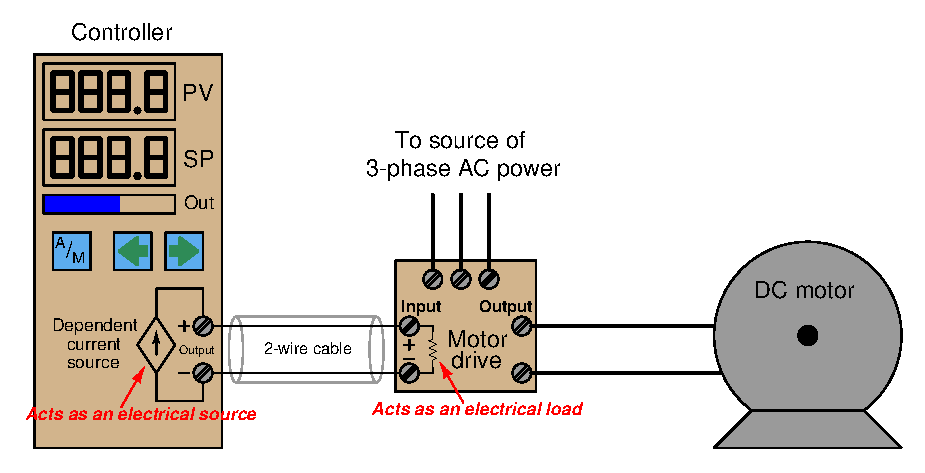
\includegraphics{current04.eps}$$

Here, the variable-speed motor drive is a high-power electronic circuit that takes 3-phase AC power in and converts it to DC power at a variable voltage (that voltage level controlled by the 4-20 mA signal from the controller output).  Another style of motor ``drive'' is one that takes in AC power and outputs 3-phase AC power at variable voltage and frequency to power an AC induction motor.  This latter style is usually called a \textit{variable frequency drive} or \textit{VFD}, but it looks the same to the controller output: a fixed resistive load accepting the 4-20 mA output signal.  \index{Variable-frequency drive}  \index{VFD}

\vskip 10pt

\filbreak

In some process applications the final control element is ``reverse-acting'' in that a controller output current value of 4 mA tells the FCE to go to its ``full'' (100\%) capacity and a controller output current value of 20 mA commands the FCE to go to its minimum (0\%) capacity.  Such is the case with an I/P transducer driving an ``air-to-close'' pneumatic control valve, where the valve's spring works to push the throttling mechanism open and air pressure on the valve diaphragm works to push the throttling mechanism shut.  A practical reason for designing a control system like this is if the dictates of process safety require the valve go wide-open if ever the instrument air supply fails or the 4-20 mA output signal circuit fails. 

In such applications, we need to configure the controller in such a way that the output display (digital read-out and/or bargraph) is \textit{reverse-indicating} so as to avoid confusing any human operator using the controller.  Since 4 mA represents a wide-open control valve and 20 mA represents a fully shut control valve, a reverse-indicating controller will display 0\% output when the current signal is 20 mA and 100\% output when the current signal is 4 mA (i.e. the controller display is a direct representation of \textit{control valve stem position}, not of the current signal itself):  \index{Reverse indication, controller output}

$$\includegraphics{current62.eps}$$

It should be noted that direct or reverse \textit{indication} on the controller's faceplate is unrelated to direct or reverse \textit{control action} of the controller's algorithm.  The former is merely the way in which the output signal is graphically represented to the human operator while the latter is the relationship between the process variable (PV) signal and the controller's output (MV) signal necessary for negative-feedback control.  For the sake of argument, this controller's automatic action could still be \textit{direct} (i.e. greater PV signal = greater output signal) even though its output bargraph indication is \textit{reverse} in order to faithfully show valve stem position to the human operator.








\filbreak
\section{4-wire (``self-powered'') transmitter current loops}

DC electric current signals may also be used to communicate process measurement information from transmitters to controllers, indicators, recorders, alarms, and other input devices.  Recall that the purpose of a \textit{transmitter} is to sense some physical variable (e.g. pressure, temperature, flow) and then report that quantity in the form of a signal, in this case a 4 to 20 milliamp DC current proportional to that measured quantity.  The simplest form of 4-20 mA measurement loop is one where the transmitter has two terminals for the 4-20 mA signal wires to connect, and two more terminals where a power source connects.  These transmitters are called ``4-wire'' or ``self-powered'' units.  The current signal from the transmitter connects to the \textit{process variable input} terminals of the controller to complete the loop: \index{4-wire transmitter} \index{Self-powered transmitter}

$$\includegraphics{current09.eps}$$

Some process controllers are not equipped to directly accept milliamp input signals, but rather can only interpret DC voltage signals.  In such cases we must connect a precision resistor across the controller's input terminals to convert the 4-20 mA transmitter signal into a standardized analog voltage signal the controller can understand.  A voltage signal range of 1 to 5 volts is standard, although some models of controller use different voltage ranges and therefore require different precision resistor values.  If the voltage range is 1-5 volts and the current range is 4-20 mA, the precision resistor value must be 250 ohms according to Ohm's Law.

Since this is a digital controller, the input voltage at the controller terminals is interpreted by an analog-to-digital converter (ADC) circuit, which converts the measured voltage into a digital number the controller's microprocessor can interpret.

\filbreak

In some installations, transmitter power is supplied through additional wires in the cable from a power source located near the controller:

$$\includegraphics{current10.eps}$$

The obvious disadvantage of this scheme is the requirement of two more conductors in the cable.  More conductors means the cable will be larger-diameter and more expensive for a given length.  Cables with more conductors will require larger electrical conduit to fit in to, and all field wiring panels will have to contain more terminal blocks to marshal the additional conductors.  If no suitable electrical power source exists at the transmitter location, though, a 4-wire cable is necessary to service a 4-wire transmitter.








\filbreak
\section{2-wire (``loop-powered'') transmitter current loops}

\label{2-wire_transmitters}

It is possible to convey electrical power \textit{and} communicate analog information over the same two wires using 4 to 20 milliamps DC, if we design the transmitter to be \textit{loop-powered}.  A loop-powered transmitter connects to a process controller with only two wires, which is why loop-powered transmitters are synonymously known as \textit{2-wire transmitters}:  \index{Loop-powered transmitter}  \index{2-wire transmitter}

$$\includegraphics{current11.eps}$$

Here, the transmitter is not really a current \textit{source} in the sense that a 4-wire transmitter is.  Instead, a 2-wire transmitter's circuitry is designed to act as a current \textit{regulator}, limiting current in the series loop to a value representing the process measurement, while relying on a remote source of power to motivate the electric current.  Please note the direction of the arrow in the transmitter's dependent current source symbol, and how it relates to the voltage polarity marks.  Refer back to the illustration of a 4-wire transmitter circuit for comparison.  The current ``source'' in this loop-powered transmitter actually behaves as an electrical \textit{load}\footnote{Some of my students have referred to such a circuit as a \textit{smart load}, since it functions as a load but nevertheless exerts control over the circuit current.}, while the current source in the 4-wire transmitter functioned as a true electrical source.

A loop-powered transmitter gets its operating power from the minimum terminal voltage and current available at its two terminals.  With the typical source voltage being 24 volts DC, and the maximum voltage dropped across the controller's 250 ohm resistor being 5 volts DC, the transmitter should always have at least 19 volts available at its terminals.  Given the lower end of the 4-20 mA signal range, the transmitter should always have at least 4 mA of current to function on.  Thus, the transmitter will always have a certain minimum amount of electrical power available on which to operate, while regulating current to signal the process measurement to the receiving instrument.

\filbreak

Internally, the electronic hardware of a 2-wire transmitter circuitry resembles the following (simplified) diagram.  Note that everything shown within the shaded rectangle is represented by the ``2-wire transmitter'' circle in the previous diagram:

$$\includegraphics{current12.eps}$$

All sensing, scaling, and output conditioning circuitry inside the transmitter must be designed to operate on less than 4 mA of DC current, and at a modest terminal voltage.  In order to create loop currents exceeding 4 mA -- as the transmitter must do in order to span the entire 4 to 20 milliamp signal range -- the transmitter circuitry uses a transistor to shunt (bypass) extra current from one terminal to the other as needed to make the total current indicative of the process measurement.  For example, if the transmitter's internal operating current is only 3.8 mA, and it must regulate loop current at a value of 16 mA to represent a condition of 75\% process measurement, the shunt transistor will be driven by the opamp to bypass exactly 12.2 mA of current (because 3.8 mA + 12.2 mA = 16.0 mA).

The very low amount of electrical power available at a 2-wire transmitter's terminals limits its functionality.  If the transmitter requires more electrical power than can be delivered with 4 milliamps and 19 volts (minimum each), the only solution is to go with a 4-wire transmitter where the power conductors are separate from the signal conductors.  An example of a process transmitter that must be 4-wire is a chemical analyzer such as a chromatograph, requiring enough power to operate an electrical heater, solenoid valves, and an on-board computer to process the sensor data.  There is simply no way to operate a machine as complex and power-hungry as a 2010-era chromatograph on 4 milliamps and 19 volts!

Early current-based industrial transmitters were not capable of operating on such low levels of electrical power, and so used a different current signal standard: 10 to 50 milliamps DC.  Loop power supplies for these transmitters ranged upwards of 90 volts to provide enough power for the transmitter.  Safety concerns made the 10-50 mA standard unsuitable for some industrial installations, and modern microelectronic circuitry with its reduced power consumption made the 4-20 mA standard practical for nearly all types of process transmitters. \index{10 to 50 mA}






\filbreak
\section{4-wire ``passive'' versus ``active'' output transmitters}

Some self-powered (4-wire) analog electronic transmitters are designed to behave as electrical loads rather than as electrical sources.  Such transmitters are commonly referred to as having \textit{passive} or \textit{sinking} 4-20 mA outputs, as opposed to the \textit{active} or \textit{sourcing} 4-wire transmitters previously described:  \index{4-wire transmitter, passive output}  \index{4-wire transmitter, active output}  \index{4-wire transmitter, sinking output}  \index{4-wire transmitter, sourcing output}

$$\includegraphics{current61.eps}$$

At first this seems needlessly confusing.  Why build a self-powered transmitter requiring a second power supply in the circuit to drive the 4-20 mA signal?  The reason for this type of transmitter's existence is the sheer popularity of loop-powered 2-wire 4-20 mA transmitters.  Loop-powered field instruments have become so popular in industry that many control systems, PLCs, indicators, and other receiving devices have their own loop power supply built in so that these systems can \textit{only} connect to loads and are therefore incompatible with current-sourcing 4-wire transmitters.  Thus, ``passive'' or ``sinking'' 4-wire transmitters were developed to accommodate control systems designed to work (only) with loop-powered instruments.

Some 4-wire transmitters are configurable for either passive or active (i.e. sinking versus sourcing) operation, requiring the installing technician to pay close attention in order for the circuit to properly function.






\filbreak
\section{Troubleshooting current loops}

A fundamental principle in instrumentation system troubleshooting is that every instrument has at least one input and at least one output, and that the output(s) should accurately correspond to the input(s).  If an instrument's output is not properly corresponding to its input according to the instrument's design function, there must be something wrong with that instrument.

Consider the inputs and outputs of several common instruments: transmitters, controllers, indicators, and control valves.  Each of these instruments takes in (input) data in some form, and generates (output) data in some form.  In any instrument ``loop,'' the output of one instrument feeds into the input of the next, such that information passes from one instrument to another.  By intercepting the data communicated between components of an instrument system, we are able to locate and isolate faults.  In order to properly understand the intercepted data, we must understand the inputs and outputs of the respective instruments and the basic functions of those instruments.

The following illustrations highlight inputs and outputs for instruments commonly found in control systems:

$$\includegraphics{trouble09.eps}$$

$$\includegraphics{trouble10.eps}$$

In order to check for proper correspondence between instrument inputs and outputs, we must be able to use appropriate test equipment to intercept the signals going into and out of those instruments.  For 4-20 mA analog signal-based instruments, this means we must be able to use electrical meters capable of accurately measuring current and voltage.





\filbreak
\subsection{Using a standard milliammeter to measure loop current}

Since the signal of interest is represented by an electric current in an instrumentation current ``loop'' circuit, the obvious tool to use for troubleshooting is a multimeter capable of accurately measuring DC milliamperes.  Unfortunately, though, there is a major disadvantage to the use of a milliammeter: the circuit must be ``broken'' at some point to connect the meter in series with the current, and this means the current will fall to 0 mA until the meter is connected (then fall to 0 mA when the meter is removed from the circuit).  Interrupting the current means interrupting the flow of information conveyed by that current, be it a process measurement or a command signal to a final control element.  This \textit{will} have adverse effects on a control system unless certain preparatory steps are taken.

Before ``breaking the loop'' to connect your meter, one must first warn all appropriate personnel that the signal will be interrupted at least twice, falling to a value of $-25$\% each time.  If the signal to be interrupted is coming from a process transmitter to a controller, the controller should be placed in Manual mode so it will not cause an upset in the process (by moving the final control element in response to the sudden loss of PV signal).  Also, process alarms should be temporarily disabled so they do not cause panic.  If this current signal also drives process shutdown alarms, these should be temporarily disabled so that nothing shuts down upon interruption of the signal.

If the current signal to be interrupted is a command signal from a controller to a final control element, the final control element either needs to be manually overridden so as to hold a fixed setting while the signal varies, or it needs to be bypasses completely by some other device(s).  If the final control element is a control valve, this typically takes the form of opening a bypass valve and closing at least one block valve:

$$\includegraphics{current05.eps}$$

Since the manually-operated bypass valve now performs the job the automatic control valve used to do, a human operator must remain posted at the bypass valve to carefully throttle it and maintain control of the process.

Block and bypass valves for a large gas flow control valve may be seen in the following photograph:

$$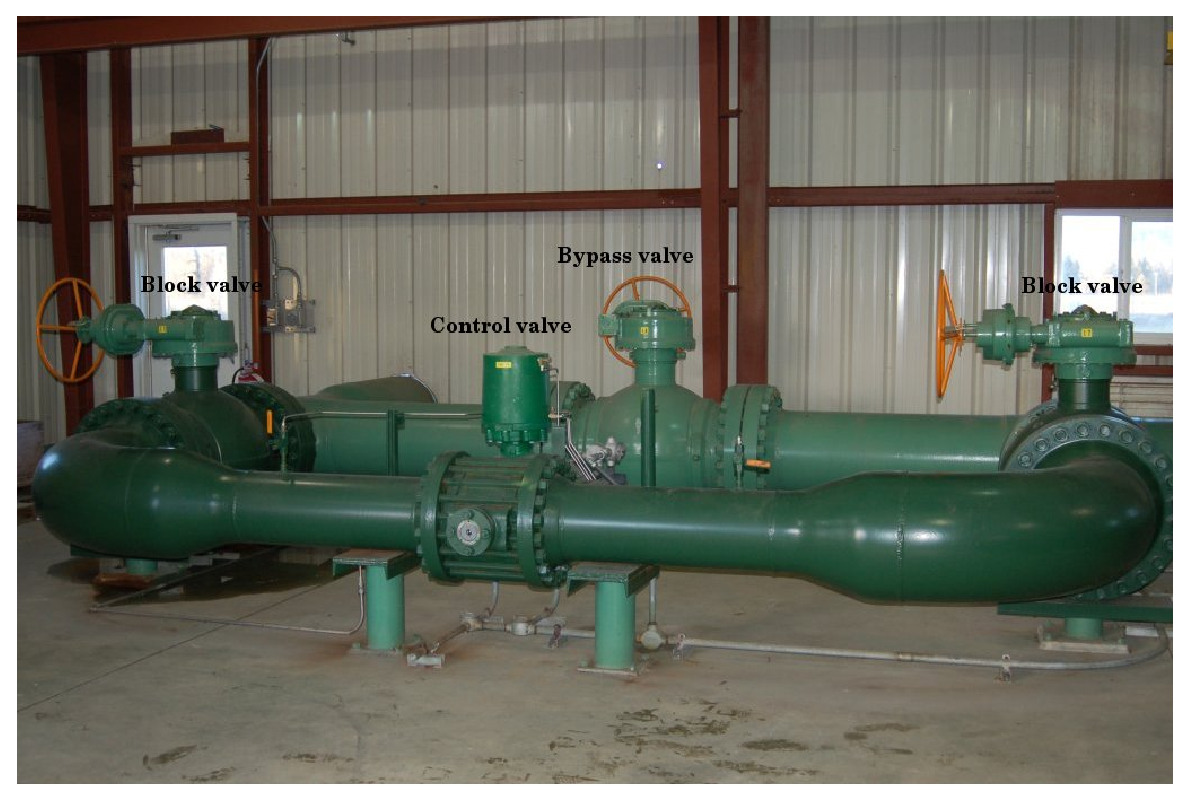
\includegraphics[width=5in]{current26.eps}$$

\vskip 10pt

In consideration of the labor necessary to safely interrupt the current signal to a control valve in a live process, we see that the seemingly simple task of connecting a milliammeter in series with a 4-20 mA current signal is not as easy as it may first appear.  Better ways must exist, no?







\filbreak
\subsection{Using a clamp-on milliammeter to measure loop current}

One better way to measure a 4-20 mA signal without interrupting it is to do so magnetically, using a clamp-on milliammeter.  Modern Hall-effect sensors are sensitive and accurate enough to monitor the weak magnetic fields created by the passage of small DC currents in wires.  Ammeters using Hall-effect sensors have are completely non-intrusive because they merely clamp around the wire, with no need to ``break'' the circuit.  An example of a such a clamp-on current meter is the Fluke model 771, shown in this photograph:  \index{Fluke model 771 clamp-on milliammeter}   \index{Clamp-on milliammeter}

$$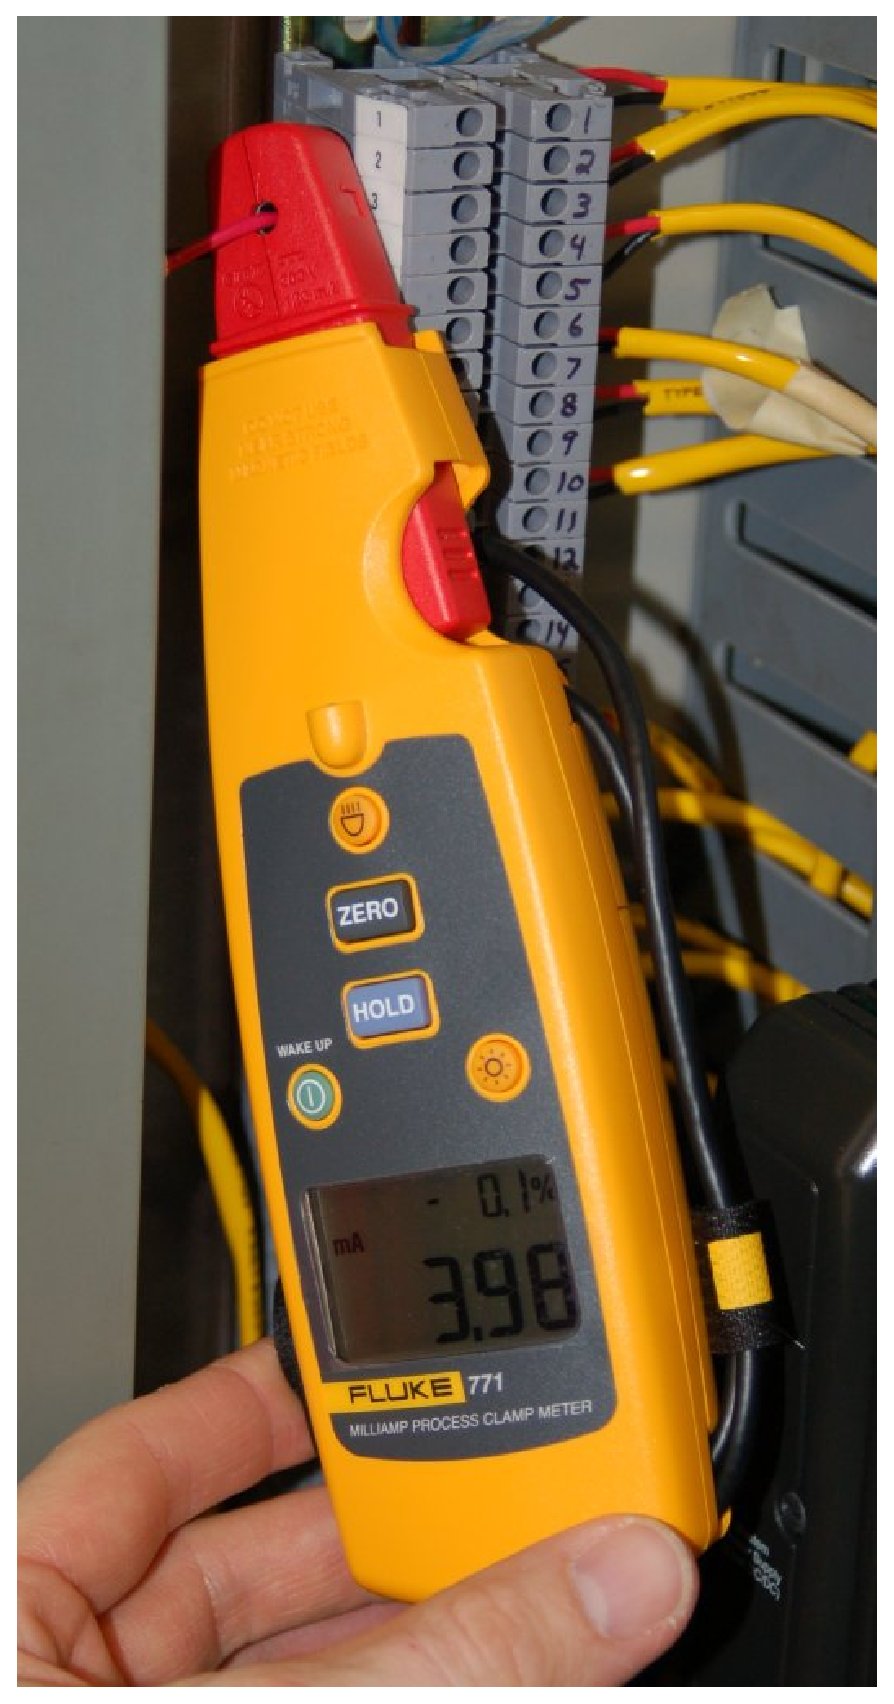
\includegraphics[width=2in]{current27.eps}$$

Note how this milliammeter not only registers loop current (3.98 mA as shown in the photograph), but it also converts the milliamp value into a percentage of range, following the 4 to 20 mA signal standard.  One disadvantage to be aware of for clamp-on milliammeters is the susceptibility to error from strong external magnetic fields.  Steady magnetic fields (from permanent magnets or DC-powered electromagnets) may be compensated for by performing a ``zero'' adjustment with the instrument held in a similar orientation prior to measuring loop current through a wire.







\filbreak
\subsection{Using ``test'' diodes to measure loop current}

Another way to measure a 4-20 mA signal without interrupting it involves the use of a rectifying diode, originally installed in the loop circuit when it was commissioned.  A ``test'' diode may be placed anywhere in series within the loop in such a way that it will be forward-biased.  During normal operation, the diode will drop approximately 0.7 volts, as is typical for any silicon rectifying diode when forward biased.  The following schematic diagram shows such a diode installed in a 2-wire transmitter loop circuit: \index{Diode, in current loop circuit}  \index{Test diode}

$$\includegraphics{current06.eps}$$

If someone connects a milliammeter in parallel with this diode, however, the very low input resistance of the ammeters ``shorts past'' the diode and prevents any substantial voltage drop from forming across it.  Without the necessary forward voltage drop, the diode effectively turns off and conducts 0 mA, leaving the entire loop current to pass through the ammeter:

$$\includegraphics{current07.eps}$$

When the milliammeter is disconnected, the requisite 0.7 volt drop appears to turn on the diode, and all loop current flows through the diode again.  At no time is the loop current ever interrupted, which means a technician may take current measurements this way and never have to worry about generating false process variable indications, setting off alarms, or upsetting the process.

Such a diode may be installed at the nearest junction box, between terminals on a terminal strip, or even incorporated into the transmitter itself.  Some process transmitters have an extra pair of terminals labeled ``Test'' for this exact purpose.  A diode is already installed in the transmitter, and these ``test'' terminals serve as points to connect the milliammeter across.  

\filbreak

The following photograph shows an example of this on a Rosemount model 3051 differential pressure transmitter:

$$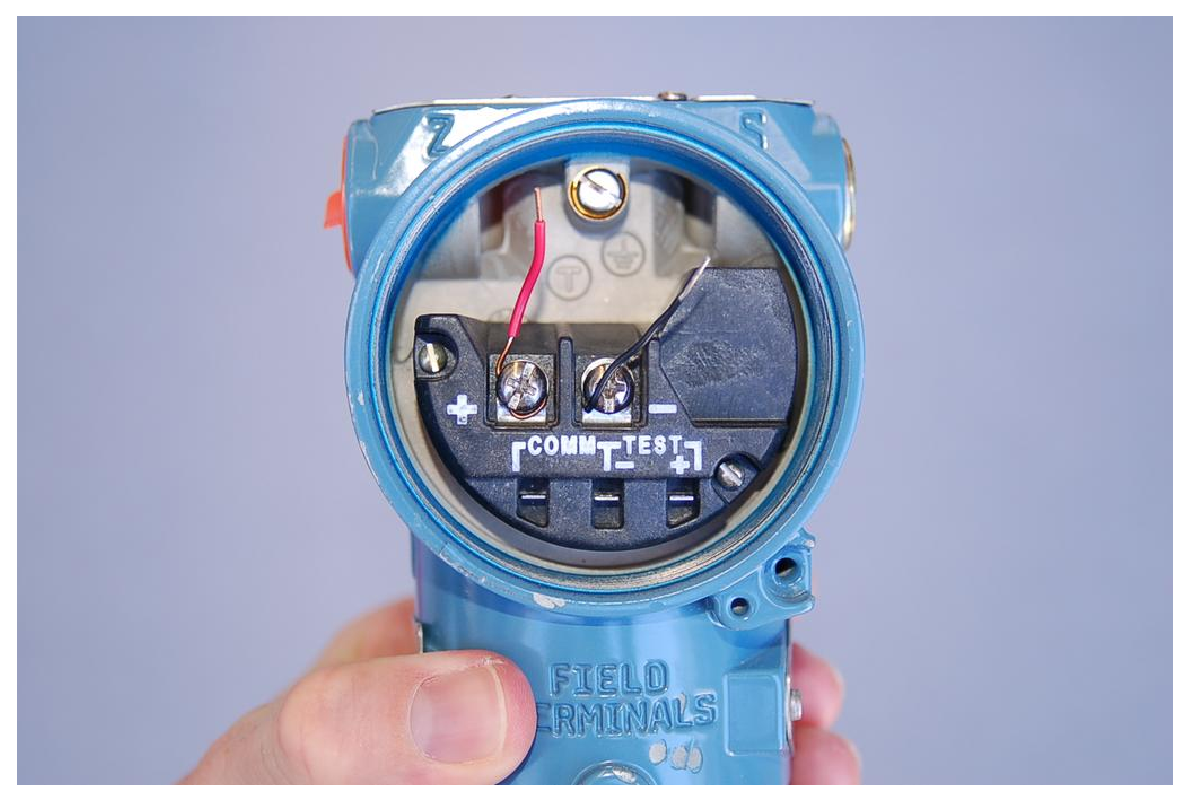
\includegraphics[width=4in]{current28.eps}$$

Note the two test points labeled ``TEST'' below and to the right of the main screw terminals where the loop wiring attaches.  Connecting an ammeter to these two test points allows for direct measurement of the 4-20 mA current signal without having to un-do any wire connections in the circuit.

Transmitters equipped with analog meter movements for direct visual indication of the 4-20 mA signal usually connect the analog milliammeter in parallel with just such a diode.  The reason for doing this is to maintain loop continuity in the event the fine-wire coil inside the milliammeter movement were to accidently break open.






\filbreak
\subsection{Using shunt resistors to measure loop current}

A similar method for non-invasively measuring current in a 4-20 mA instrumentation circuit is to install a precision resistor in series.  If the resistance value is precisely known, the technician merely needs to measure voltage across it with a voltmeter and use Ohm's Law to calculate current:

$$\includegraphics{current08.eps}$$

In electronics, such a precision resistor used for measuring current is often referred to as a \textit{shunt} resistor.  Shunt resistor values are commonly very small, for their purpose is to assist in current measurement without imposing undue voltage drop within a circuit.  It is rare to find a 250 ohm resistor used strictly as a diagnostic shunt resistor, because the extra voltage drop (1 to 5 volts, depending on the current signal level) may ``starve'' loop-powered instruments of voltage necessary to operate.  Shunt resistor values as low as 1 ohm may be found installed in 4-20 mA current loops at strategic locations where technicians may need to measure loop current\footnote{Of course, a 1 ohm resistor would drop 4 mV at 4 mA loop current, and drop 20 mV at 20 mA loop current.  These small voltage values necessitate a highly accurate DC voltmeter for field measurement!}.  \index{Shunt resistor}








\filbreak
\subsection{Troubleshooting current loops with voltage measurements}

If neither component (diode nor shunt resistor) is pre-installed in the circuit, and if a Hall-effect (clamp-on) precision milliammeter is unavailable, a technician may still perform useful troubleshooting measurements using nothing but a DC voltmeter.  Here, however, one must be careful of how to interpret these voltage measurements, for they may not directly correspond to the loop current as was the case with measurements taken in parallel with the precision resistor.

Take for example this 4-20 mA loop where a controller sends a command signal to an I/P transducer: \index{I/P transducer}

$$\includegraphics{current03.eps}$$

There is no standardized resistance value for I/P transducer coils, and so the amount of voltage dropped across the I/P terminals for any given amount of loop current will be unique for every different model of I/P.  The Fisher model 567 I/P transducer built for 4-20 mA signals has a normal coil resistance of 176 ohms.  Thus, we would expect to see a voltage drop of approximately 0.7 volts at 4 mA and a drop of approximately 3.5 volts at 20 mA across the I/P terminals.  Since the controller output terminals are directly in parallel with the I/P terminals, we would expect to see approximately the same voltage there as well (slightly greater due to wire resistance).  The lack of known precision in the I/P coil resistance makes it difficult to tell exactly how much current is in the loop for any given voltage measurement we take with a voltmeter.  However, if we do know the approximate coil resistance of the I/P, we can at least obtain an estimate of loop current, which is usually good enough for diagnostic purposes.  

If the I/P coil resistance is completely unknown, voltage measurements become useless for quantitative determination of loop current.  Voltage measurements would be useful only for qualitatively determining loop continuity (i.e. whether there is a break in the wiring between the controller and I/P).

\filbreak

Another example for consideration is this loop-powered 4-20 mA transmitter and controller circuit, where the controller supplies DC power for the loop:

$$\includegraphics{current13.eps}$$

It is very common to find controllers with their own built-in loop power supplies, due to the popularity of loop-powered (2-wire) 4-20 mA transmitters.  If we know the transmitter requires a DC voltage source somewhere in the circuit to power it up, it makes sense to include one in the controller, right?

The only voltage measurement that directly and accurately corresponds to loop current is the voltage directly across the 250 ohm precision resistor.  A loop current of 4 mA will yield a voltage drop of 1 volt, 12 mA will drop 3 volts, 20 mA will drop 5 volts, etc.  

A voltage measurement across the transmitter terminals will show us the \textit{difference} in voltage between the 26 volt power supply and the voltage dropped across the 250 ohm resistor.  In other words, the transmitter's terminal voltage is simply what is left over from the source voltage of 26 volts after subtracting the resistor's voltage drop.  This makes the transmitter terminal voltage inversely proportional to loop current: the transmitter sees approximately 25 volts at 4 mA loop current (0\% signal) and approximately 21 volts at 20 mA loop current (100\% signal).

The use of the word ``approximate'' is very intentional here, for loop power supplies are usually non-regulated.  In other words, the ``26 volt'' rating is approximate and subject to change!  One of the advantages of the loop-powered transmitter circuit is that the source voltage is largely irrelevant, so long as it exceeds the minimum value necessary to ensure adequate power to the transmitter.  If the source voltage drifts for any reason, it will have no impact on the measurement signal at all, because the transmitter is built as a \textit{current regulator}, regulating current in the loop to whatever value represents the process measurement, regardless of slight changes in loop source voltage, wire resistance, etc.  This rejection of power supply voltage changes means the loop power supply need not be regulated, and so in practice it rarely is.

This brings us to a common problem in loop-powered 4-20 mA transmitter circuits: maintaining sufficient operating voltage at the transmitter terminals.  Recall that a loop-powered transmitter relies on the voltage dropped across its terminals (combined with a current of less than 4 mA) to power its internal workings.  This means the terminal voltage must not be allowed to dip below a certain minimum value, or else the transmitter will not have enough electrical power to continue its normal operation.  This makes it possible to ``starve'' the transmitter of voltage if the loop power supply voltage is insufficient, and/or if the loop resistance is excessive.  

To illustrate how this can be a problem, consider the following 4-20 mA measurement loop, where the controller supplies only 20 volts DC to power the loop, and an indicator is included in the circuit to provide operators with a field-mounted indication of the transmitter's measurement:

$$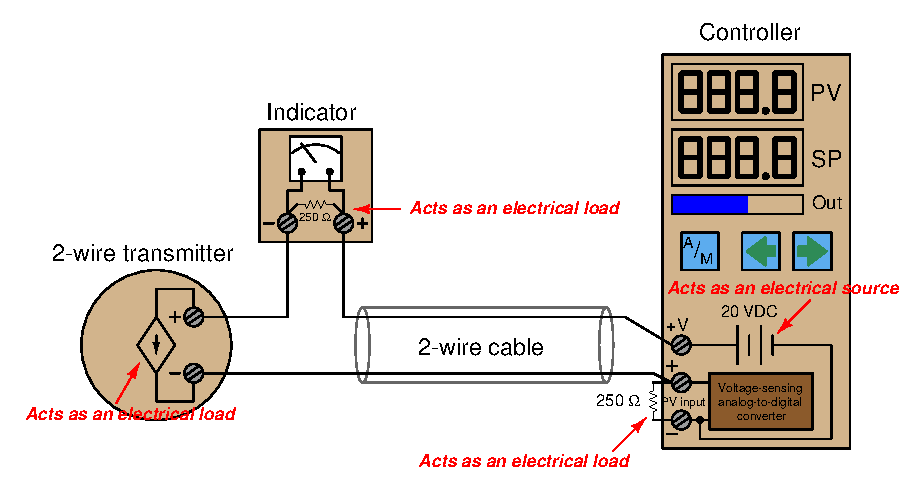
\includegraphics{current14.eps}$$

The indicator contains its own 250 ohm resistor to provide a 1-5 volt signal for the meter mechanism to sense.  This means the total loop resistance has now risen from 250 ohms to 500 ohms (plus any wire resistance).  At full current (20 mA), this total circuit resistance will drop (at least) 10 volts, leaving 10 volts or less at the transmitter terminals to power the transmitter's internal workings.  10 volts may not be enough for the transmitter to successfully operate, though.  The Rosemount model 3051 pressure transmitter, for example, requires a minimum of 10.5 volts at the terminals to operate. \index{Rosemount model 3051 differential pressure transmitter}

However, the transmitter \textit{will} operate just fine at lower loop current levels.  When the loop current is only 4 mA, for example, the combined voltage drop across the two 250 ohm resistors will be only 2 volts, leaving about 18 volts at the transmitter terminals: more than enough for practically any model of 4-20 mA loop-powered transmitter to successfully operate.  Thus, the problem of insufficient supply voltage only manifests itself when the process measurement nears 100\% of range.  This could be a difficult problem to diagnose, since it appears only during certain process conditions and not others.  A technician looking only for wiring faults (loose connections, corroded terminals, etc.) would never find the problem.

When a loop-powered transmitter is starved of voltage, its behavior becomes erratic.  This is especially true of ``smart'' transmitters with built-in microprocessor circuitry.  If the terminal voltage dips below the required minimum, the microprocessor circuit shuts down.  When the circuit shuts down, the current draw decreases accordingly.  This causes the terminal voltage to rise again, at which point the microprocessor has enough voltage to start up.  As the microprocessor ``boots'' back up again, it increases loop current to reflect the near-100\% process measurement.  This causes the terminal voltage to sag, which subsequently causes the microprocessor to shut down again.  The result is a slow on/off cycling of the transmitter's current, which makes the process controller think the process variable is surging wildly.  The problem disappears, though, as soon as the process measurement decreases enough that the transmitter is allowed enough terminal voltage to operate normally. \index{Smart transmitter}






\filbreak
\subsection{Using loop calibrators}

Special-purpose electronic test instruments called \textit{loop calibrators} exist for the express purpose of 4-20 mA current loop circuit troubleshooting.  These versatile instruments are generally capable of not only measuring current, but also \textit{sourcing} current to unpowered devices in a loop, and also \textit{simulating} loop-powered 4-20 mA transmitters.  \index{Loop calibrator}  \index{Calibrator, loop}

A very popular loop calibrator unit is the Altek model 334A, a battery-powered, hand-held unit with a rotary knob for current adjustment and toggle switches for mode setting.  The following illustration shows how this calibrator would be used to measure current in a functioning input signal loop\footnote{In the following illustrated examples, the transmitter is assumed to be a pressure transmitter with a calibrated range of 0 to 750 inches of water column, 4-20 mA.  The controller's PV (process variable) display is appropriately ranged to display 0 to 750 as well.}: \index{Altek model 334A loop calibrator}

$$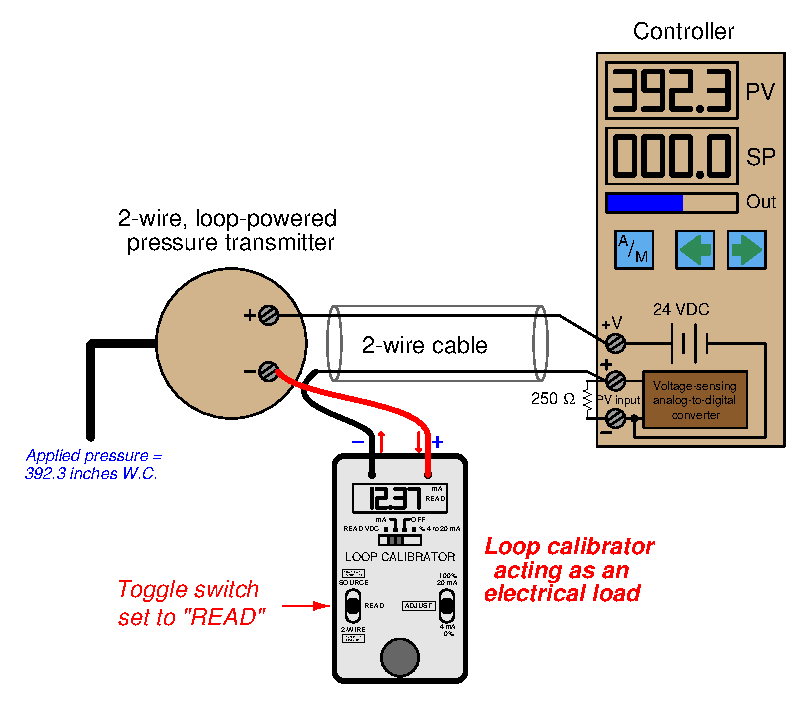
\includegraphics{current29.eps}$$

Here, the loop wiring is broken at the negative terminal of the loop-powered transmitter, and the calibrator connected in series to measure current.  If this loop had a test diode installed, the calibrator could be connected in parallel with the diode to achieve the same function.  Note the polarity of the calibrator's test leads in relation to the circuit being tested: the calibrator is acting as a passive device (i.e. as a \textit{load} rather than as a \textit{source}), with the more positive loop terminal connected to the calibrator's red test lead and the more negative terminal connected to the black test lead.

\vskip 10pt

The same loop calibrator may be used to \textit{source} (or \textit{drive}) a 4-20 mA signal into an indicating instrument to test the function of that instrument independently.  Here, we see the Altek calibrator used as a current source to send a 16.00 mA signal to the PV (process variable) input of the controller, in order to check that the controller properly senses and displays the analog current signal:

$$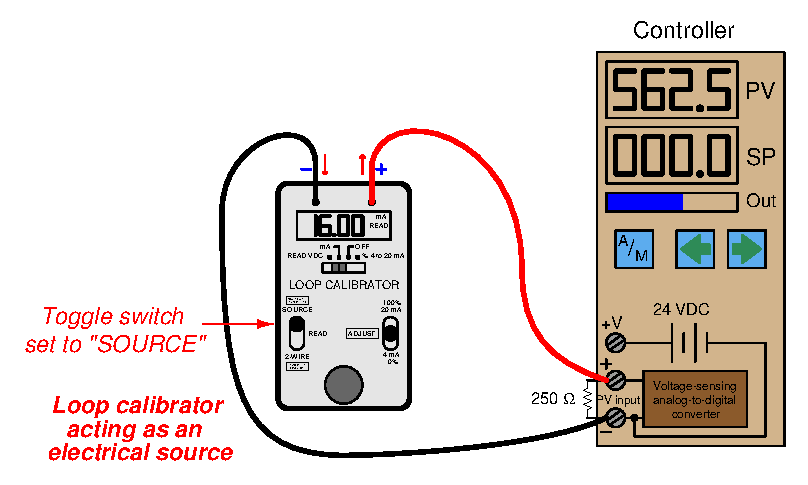
\includegraphics{current30.eps}$$

No transmitter need be included in this illustration, because the calibrator takes its place.  Note how the calibrator functions here as an active \textit{source} of current rather than a passive load as it was in the last example.  Not only does it supply the information (i.e. regulate the current), but it also provides the energy in the circuit.  The DC power source inside the controller is not used for loop power, because the calibrator in ``source'' mode provides the necessary power to drive current through the 250 ohm resistor.

\filbreak

A very common use of a loop calibrator in ``source'' mode is to test a control valve for proper calibration, quick response, and to measure friction.  Here, the loop calibrator takes place of the loop controller output, serving as the sole source of current to the I/P transducer:

$$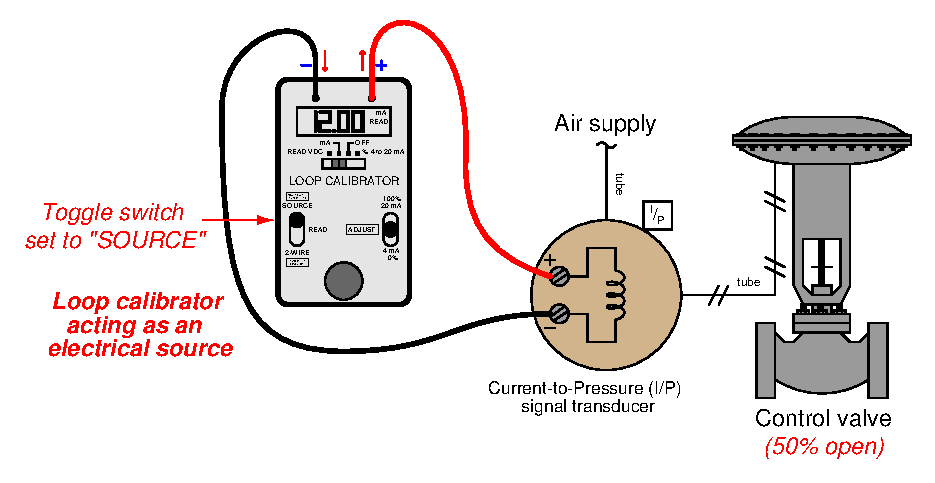
\includegraphics{current57.eps}$$

This circuit configuration is extremely useful to any instrument technician testing the response of a control valve, because it allows the signal to be finely adjusted while in the direct presence of the valve to monitor its motion.  If a control valve is suspected of having excessive friction in its moving parts, for instance, a technician may test the valve by incrementing and decrementing the loop calibrator's source current in progressively smaller steps.  Large step-changes in current should cause the valve to overcome friction and move, but small step-changes will fail to move the valve mechanism when frictional forces exceed the incremental forces produced by the changing pressure.

\filbreak

A photograph showing this very use of a loop calibrator in a valve rebuild shop appears here:

$$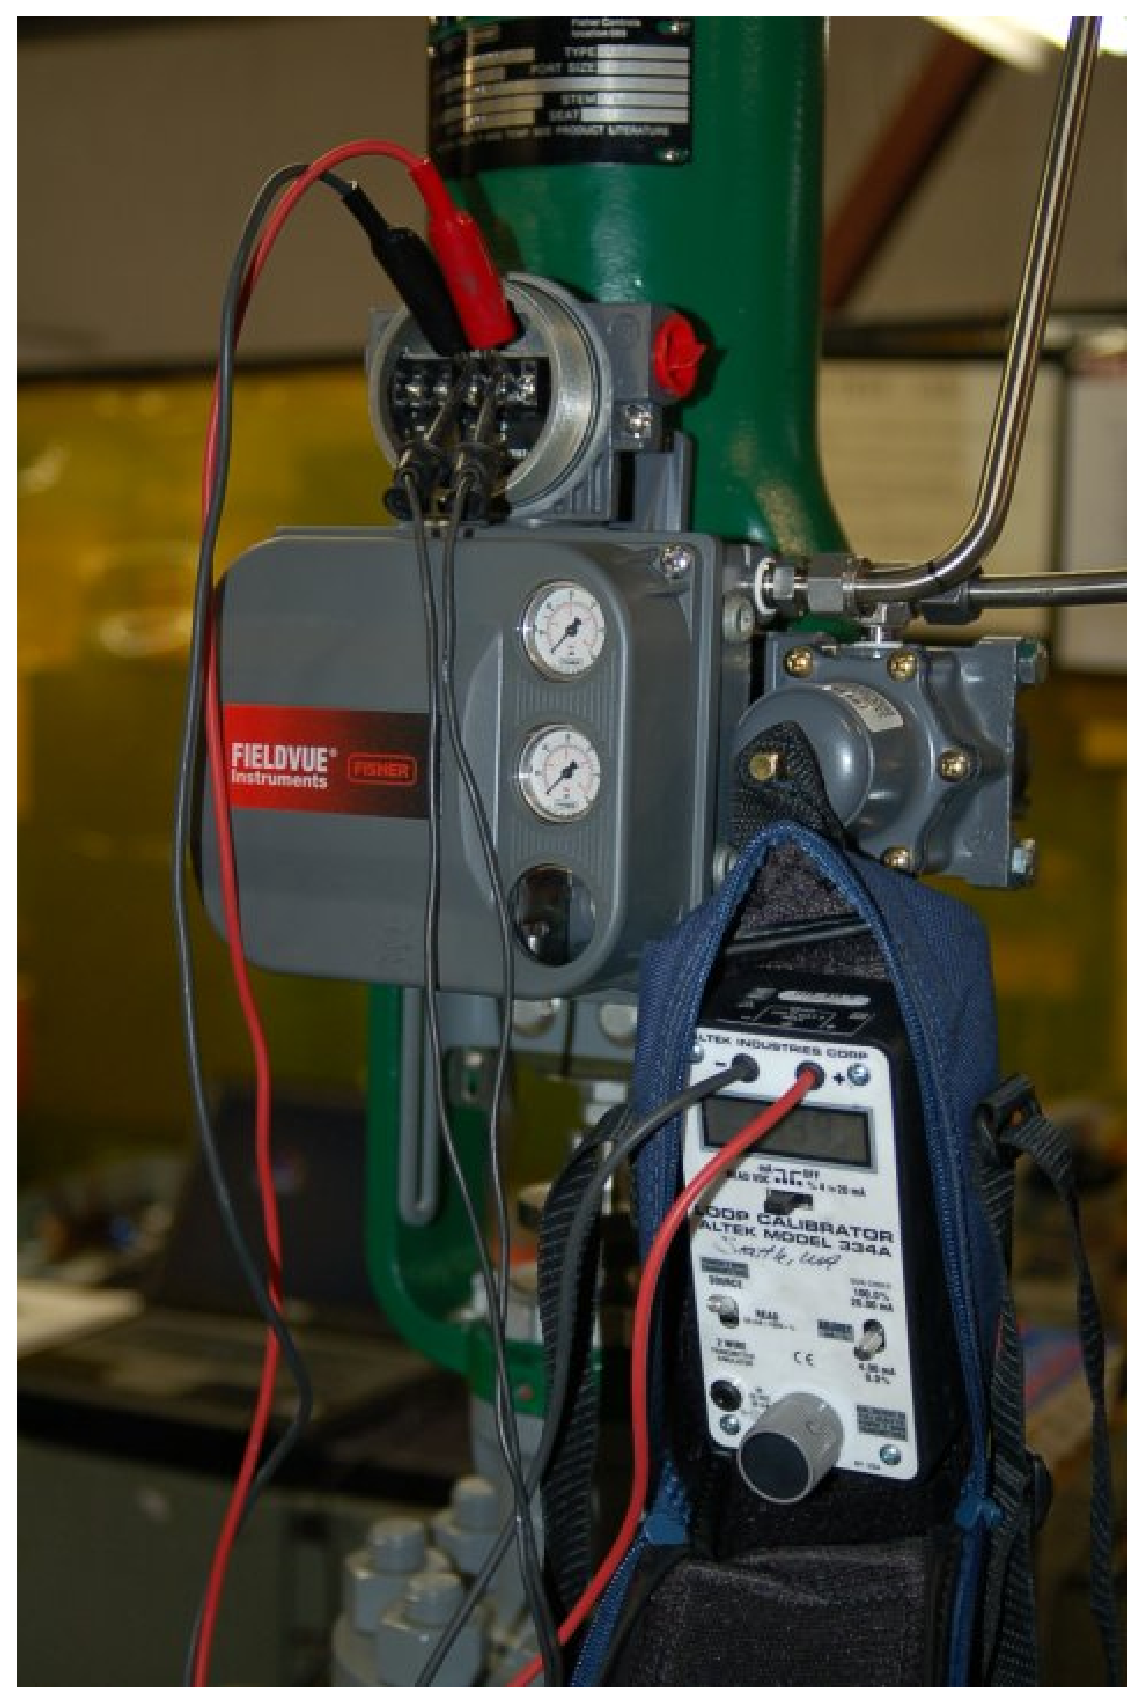
\includegraphics[height=5in]{current58.eps}$$

In this particular example, the loop calibrator connects to a device on the control valve called a \textit{positioner}, which is a more sophisticated device than an I/P transducer.  In addition to converting a 4-20 mA signal into an air pressure, the positioner also actively monitors the valve stem's position to ensure it goes to the correct position for any given 4-20 mA command signal.  Here, the technician is using the loop calibrator to verify the control valve faithfully obeys the command signal through the entire 4 to 20 milliamp signal range.

\filbreak

An alternative method of sending a known current signal into an indicating instrument providing loop power is to set the loop calibrator such that it mimics (or \textit{simulates}) the behavior of a loop-powered (2-wire) transmitter.  In this mode, the calibrator regulates loop current at a user-determined value, but provides no motivating voltage to drive this current.  Instead, it passively relies on the loop's regular voltage source to provide the necessary power:

$$\includegraphics{current31.eps}$$

Note the polarity of the calibrator's test leads: current entering the red lead and exiting the black lead, behaving as an electrical \textit{load} just the same as a loop-powered transmitter.  Like a 2-wire transmitter, the calibrator in simulate mode regulates the circuit current while depending on an external voltage source for energy.  

A loop calibrator's \textit{simulate transmitter} mode is especially useful for testing the transmitter cable and controller input to ensure any 4-20 mA signal sent by a transmitter will be correctly received and displayed by the controller.  This sort of test is commonly performed on newly-installed control systems as part of the commissioning procedure, prior to start-up of the controlled process, in order to verify the controller's process variable input, 24 VDC power supply, and transmitter wiring are all properly functioning.  Typically an instrument technician would simulate several different current values (e.g. 4 mA, 8 mA, 12 mA, 16 mA, 20 mA) with the calibrator in ``simulate'' mode while someone else monitors the controller's PV display and alarms to check for proper function.

\vskip 10pt

\filbreak

A legacy loop calibrator still familiar to many instrument technicians at the time of this writing is the classic Transmation model 1040:  \index{Transmation model 1040 loop calibrator}

$$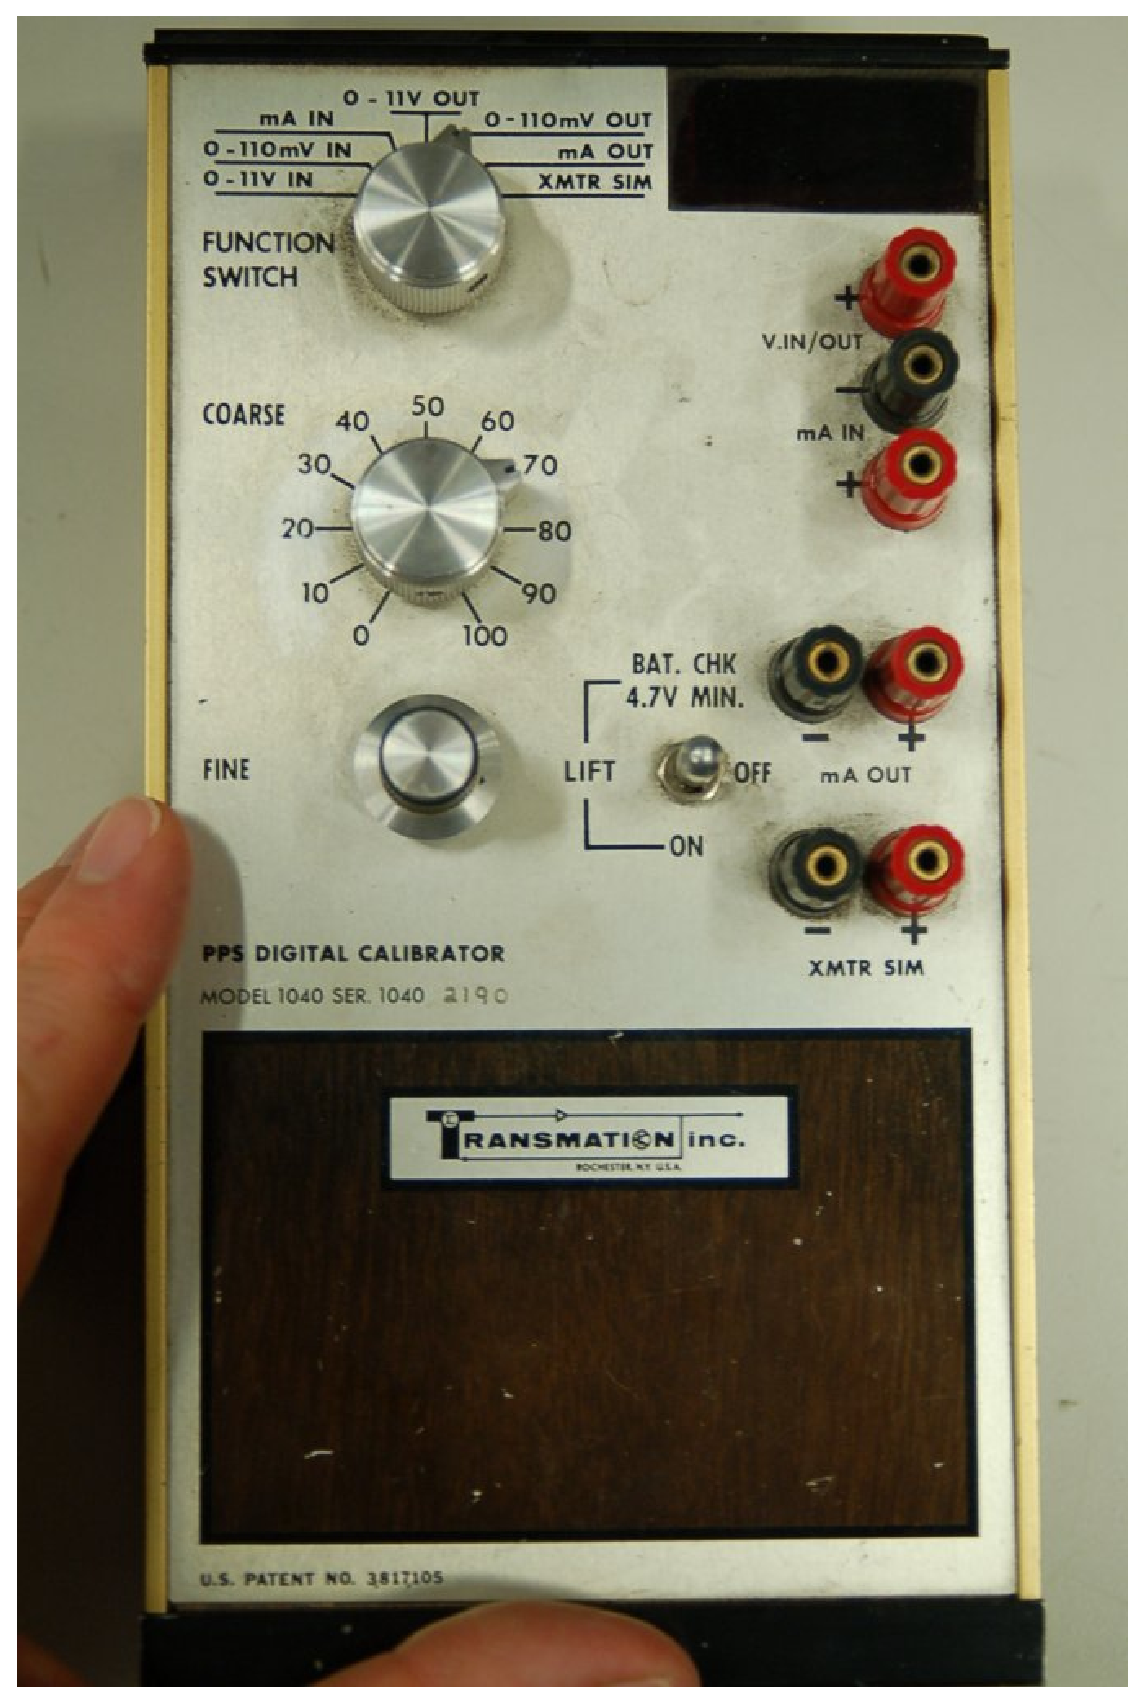
\includegraphics[width=3in]{current32.eps}$$

\filbreak

Other examples of vintage loop calibrator technology include the Nassau model 8060 (left) and the Biddle Versa-Cal (right):  \index{Nassau model 8060 loop calibrator}  \index{Biddle Versa-Cal loop calibrator}

$$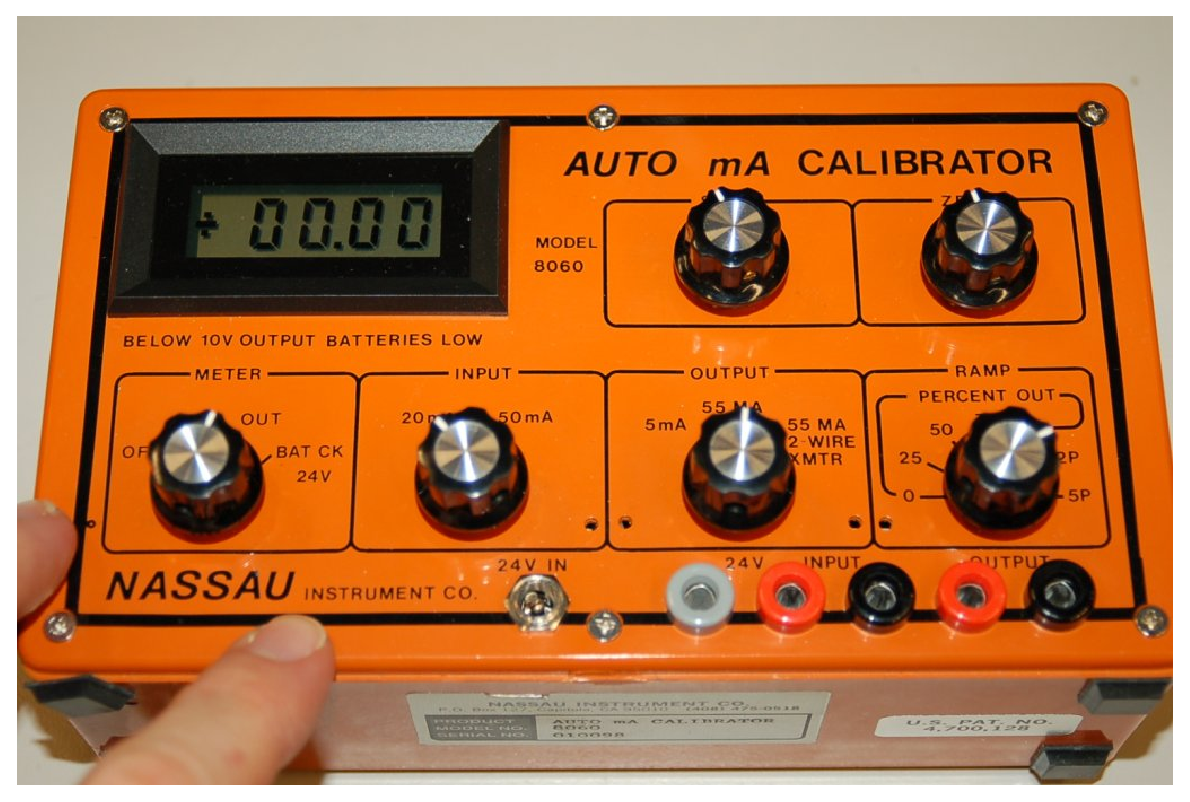
\includegraphics[width=2.5in]{current33.eps} \hskip 30pt 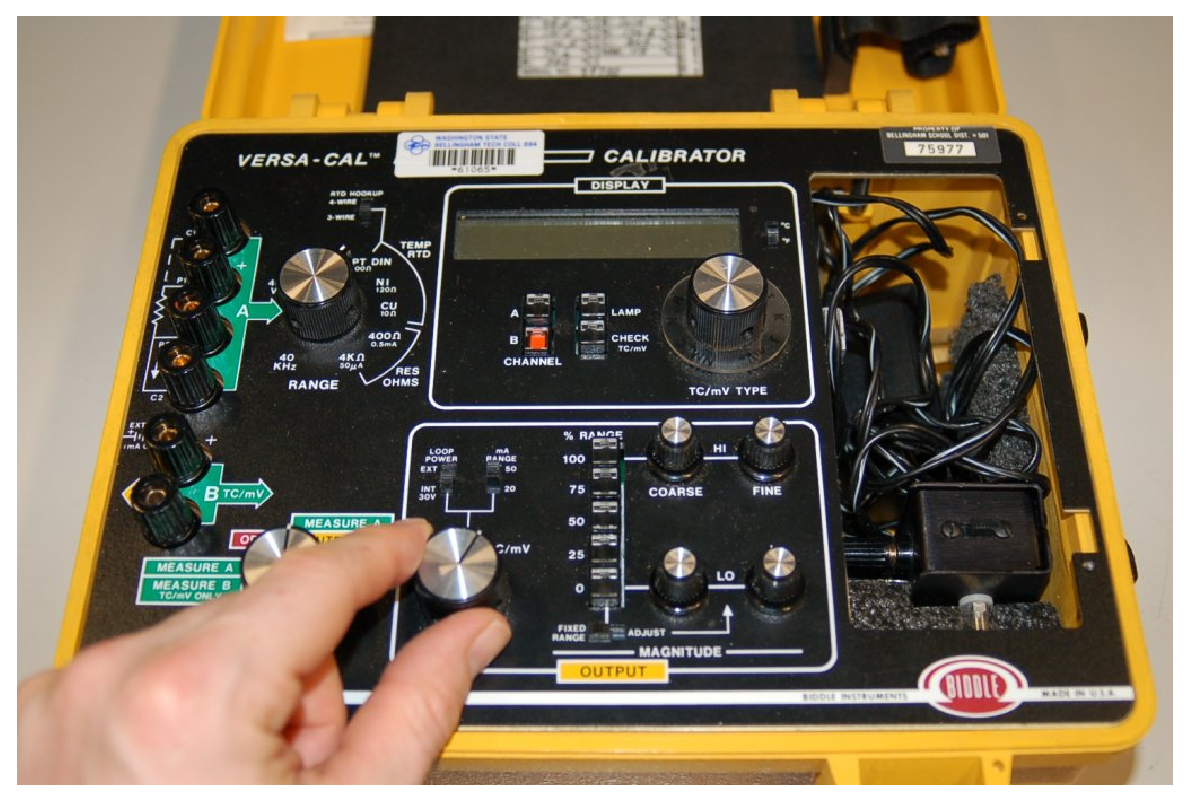
\includegraphics[width=2.5in]{current34.eps}$$

\filbreak

A modern loop calibrator manufactured by Fluke is the model 705:

$$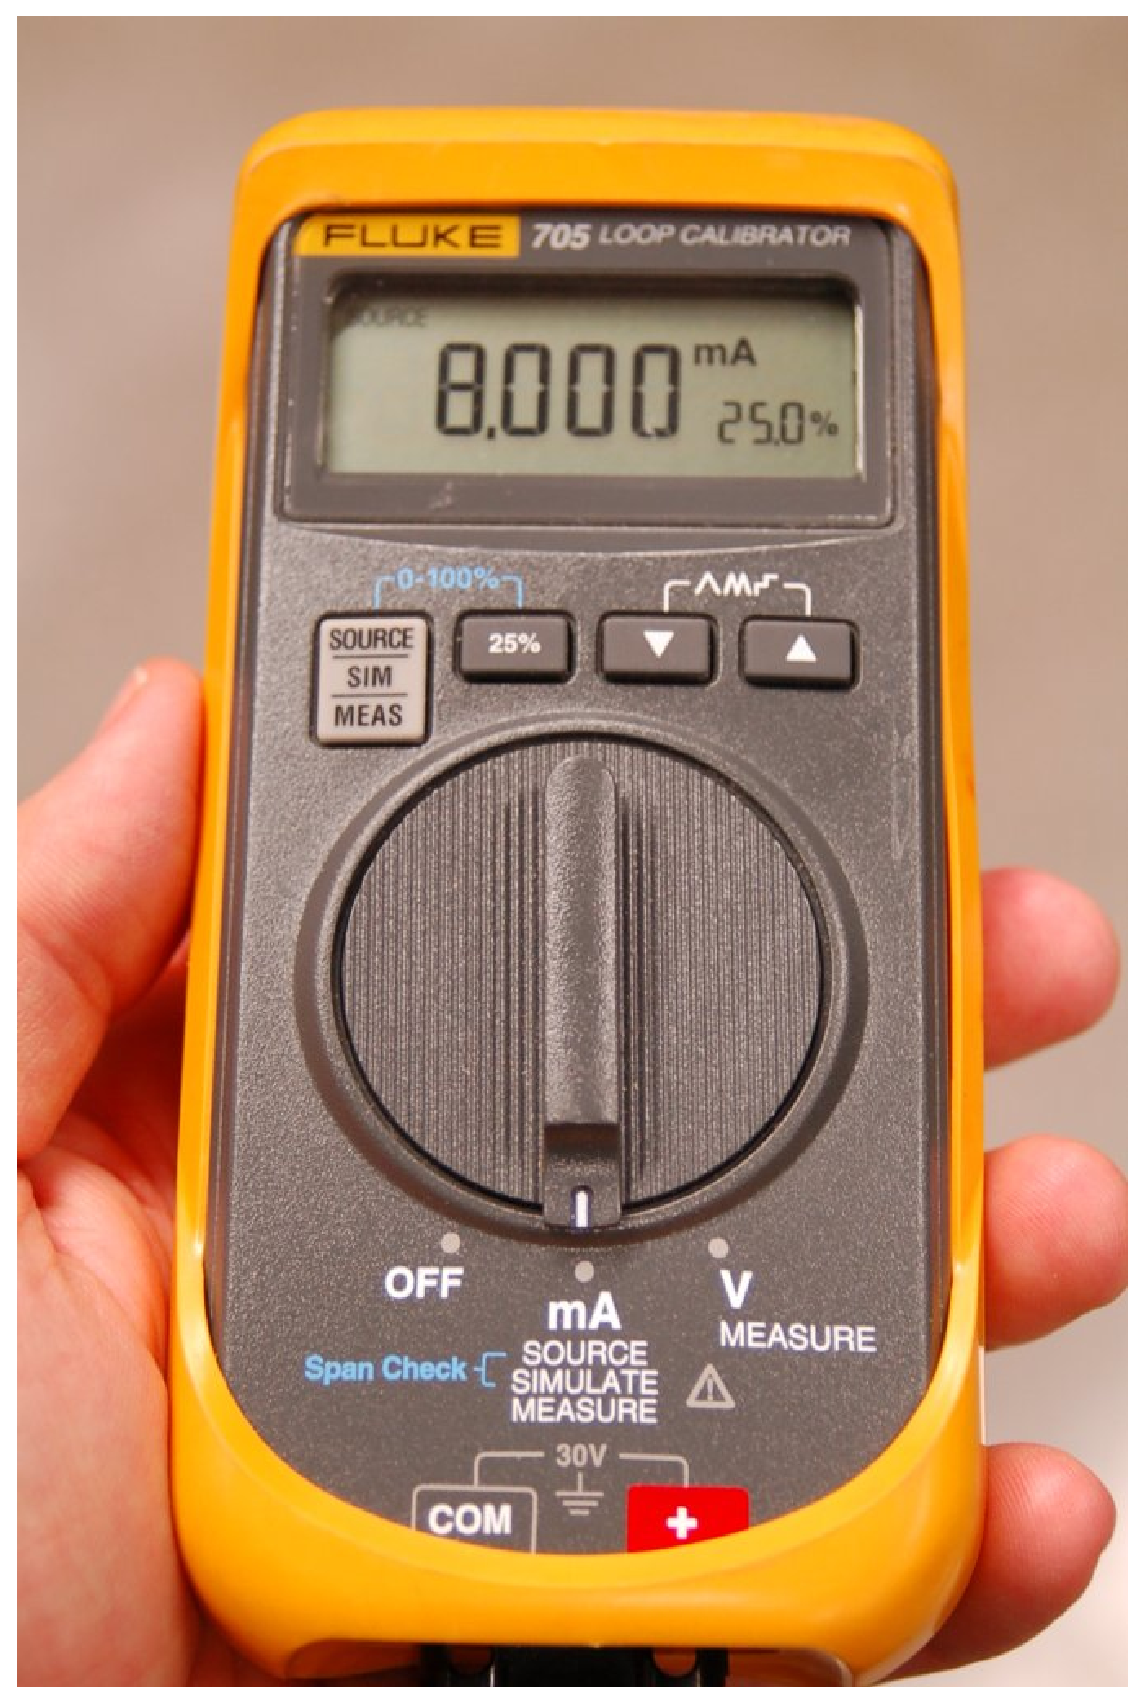
\includegraphics[width=3in]{current35.eps}$$

With this calibrator, the \textit{measure}, \textit{source}, and \textit{simulate} modes are accessed by repeatedly pushing a button, with the current mode displayed on the screen:

$$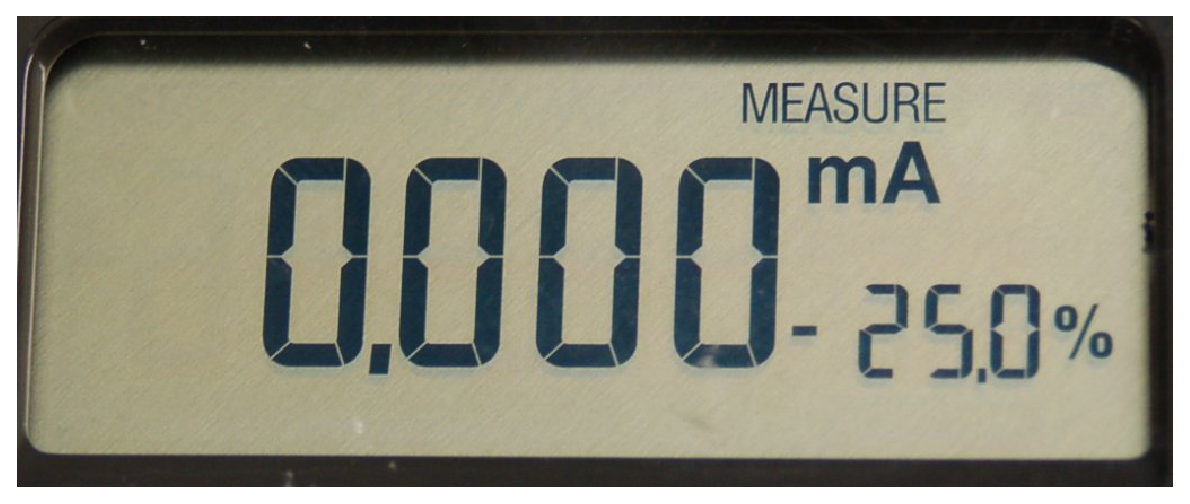
\includegraphics[width=1.5in]{current36.eps} \hskip 15pt 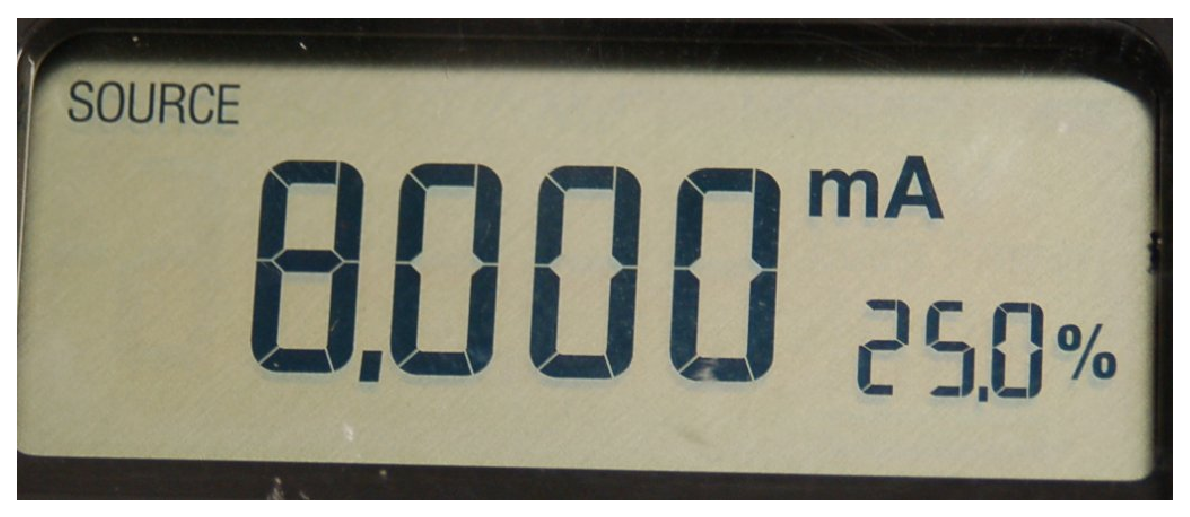
\includegraphics[width=1.5in]{current37.eps} \hskip 15pt \includegraphics[width=1.5in]{current38.eps}$$

Note the dual-numeric display, showing both loop current and percentage (assuming a 4-20 mA range).










\filbreak
\subsection{NAMUR signal levels}

One of the intrinsic benefits of a ``live zero'' analog signal standard such as 4-20 mA is that a wire break (open fault) can immediately be detected by the absence of current in the circuit.  If the signal scale started at zero (e.g. 0-20 mA), there would be no way to electrically distinguish between a broken wire and a legitimate 0\% signal value.  In other words, the ``live'' LRV point of a 4-20 mA signal provides us with a way to indicate a certain type of circuit fault in addition to indicating an analog measurement during normal operation.

The \textit{NAMUR} signal standard takes this philosophy one step further by defining specific diagnostic meaning to values of current lying outside the 4-20 mA range:  \label{NAMUR_signal_levels}

% I use comments (%) instead, so that TeX doesn't choke.

$$\vbox{\offinterlineskip
\halign{\strut
\vrule \quad\hfil # \ \hfil & 
\vrule \quad\hfil # \ \hfil \vrule \cr
\noalign{\hrule}
%
% First row
\textbf{Signal level} & \textbf{Fault condition} \cr
%
\noalign{\hrule}
%
% Another row
Output $\leq$ 3.6 mA & Sensing transducer failed low \cr
%
\noalign{\hrule}
%
% Another row
3.6 mA $<$ Output $<$ 3.8 mA & Sensing transducer failed (detected) low \cr
%
\noalign{\hrule}
%
% Another row
3.8 mA $\leq$ Output $<$ 4.0 mA & Measurement under-range \cr
%
\noalign{\hrule}
%
% Another row
21.0 $>$ Output $\geq$ 20.5 mA & Measurement over-range \cr
%
\noalign{\hrule}
%
% Another row
Output $\geq$ 21.0 mA & Sensing transducer failed high \cr
%
\noalign{\hrule}
} % End of \halign 
}$$ % End of \vbox

NAMUR-compliant transmitters are designed to limit their output signals between 3.8 mA and less than 21 mA when functioning properly.  Signals lying outside this range indicate some form of failure has occurred within the transmitter or the circuit wiring.

NAMUR-compliant control systems will recognize these errant milliamp values as fault states, and may be programmed to take specific action upon receiving these signal values.  Such actions include forcing controllers into manual mode, initiating automatic shutdown procedures, or taking some other form of safe action appropriate to the knowledge of a failed process transmitter.








\filbreak
\section{Review of fundamental principles}

Shown here is a partial listing of principles applied in the subject matter of this chapter, given for the purpose of expanding the reader's view of this chapter's concepts and of their general inter-relationships with concepts elsewhere in the book.  Your abilities as a problem-solver and as a life-long learner will be greatly enhanced by mastering the applications of these principles to a wide variety of topics, the more varied the better.

\begin{itemize}
\item \textbf{Linear equations}: any function represented by a straight line on a graph may be represented symbolically by the slope-intercept formula $y = mx + b$.  Relevant to instrument input/output scaling.
\item \textbf{Electrical sources versus loads}: electrical power sources output current (conventional flow) on their positive terminals and input current on their negative terminals (e.g. batteries and generators).  Electrical loads do the opposite (e.g. resistors).  Relevant to determining voltage drops and current directions in analog current loop circuits, as well as matching polarities between field instruments and controllers.
\item \textbf{Voltage versus current sources}: voltage sources try to maintain constant voltage with variable current, while current sources try to maintain constant current with variable voltage.  Relevant to the operation of 4-20 mA signaling circuits: loop transmitter act as current sources (or in some cases as current regulators), dropping as much or as little voltage as needed to maintain the desired amount of current in the circuit.
\item \textbf{Self-balancing opamp circuits}: all self-balancing operational amplifier circuits work on the principle of negative feedback maintaining a nearly zero differential input voltage to the opamp.  Making the ``simplifying assumption'' that the opamp's differential input voltage is exactly zero assists in circuit analysis, as does the assumption that the input terminals draw negligible current.
\end{itemize}







\filbreak
\section*{References}

% In alphabetical order!
% \noindent
% Lastname, Firstname MiddleI., \textit{Book Title}, Publisher, City, State, Year.
% \vskip 10pt
% \noindent
% Lastname, Firstname MiddleI., \textit{Book Title}, Publisher, City, State, Year.
% etc . . .

\noindent
``Designing a 4-20mA Current Loop Using the MAX1459 Sensor Signal Conditioner'' application note 1064, Maxim Integrated Products, 2005.  

\vskip 10pt

\noindent
Lipt\'ak, B\'ela G. et al., \textit{Instrument Engineers' Handbook -- Process Software and Digital Networks}, Third Edition, CRC Press, New York, NY, 2002.

\vskip 10pt

\noindent
``NAMUR'' whitepaper, Emerson Process Management, 2007.



















%%%%%%%%%%%%%%%%%%%%%%%%%%%%%%%%%%%%%%%%%%%%%%%%%%%%

